\section{Discussion}
\label{Discussion}
%\textbf{: La conclusione la incorporo come subsection della discussion o la tengo separata? }\\
In this section we discuss the results of the transformation, its feasibility and the possible future developments. We also present a use case to show how the generator works on a simple transformation.
\subsection{Emulate a BPEL Orchestration in Java}
\label{sec:OrchestrEmulation}
Emulating simple BPEL workflows in Java is possible, and we show that this is feasible in a automatized manner. Apart of the obvious constraints we have set in terms of the use of a subset of BPEL and the focus on only one pattern (see Section \ref{sec:actvitiesSubset} and \ref{sec:DesignBPELPattern}), and the difficulties to gather data from the WSDL files (see Section \ref{sec:IssueInputFiles}), the automatic transformation shows some promising features and there seems to be much ground from improvements.
A good feature is the possibility of recreating in Java the static structure of variables (messages) and participants (partnerLinks, client). The reuse of the \textit{wsimport} (Section \ref{sec:WSDLMEssagesStructure}) tool and the generic template to create partnerLink STUBs (Section \ref{sec:extrenalResources}), permits to create the representation of the static structure of elements used by the BPEL process. This eventually allows to concentrate only in the translation of the behaviour: the BPEL logic contained in the \textit{sequence} activity \ref{sec:mimicBPELLogic}. Moreover, this also abstracts our generator from the kind of web services used: it does not matter which kind of input or output the web service is able to deal with; the variables are seen as \textit{messages}, and the types do not need to be specified until it comes to Java assignation.

At the same time, once the structure has been decoupled from the behaviour, it becomes easy to think of including other BPEL patterns, because everything seems to boil done at reproducing the sequence of BPEL activities with Java method calls. 
% Our purpose was to show the feasibility of an automatic transformation from a BPEL orchestrated process to a Java application. With the use of a model-to-text methodology we met the intent and we provide a simple implementation to endorse our proof of concept.
% On the functionality of the transformation, obvious constraints have been set. First, not to overcome the complexity due to the wide structure of the BPEL language, we use a subset of the language. Second, we limit the focus to only one workflow pattern. 
% These constraints have been set not to overcome the project time-frame.


\subsection{Use Case}
\label{sec:UseCase}
Here we provide a simple use case to show how the generator works. Figure \ref{fig:GeneratorUseCase} represents a scenario where a user inputs a BPEL model and receives in output the Java application mimicing the BPEL orchestration.
The use case can be described as follows:
\begin{itemize}
 \item The runs the generator, which includes:
  \subitem Insert a BPEL input (complying with out pattern) 
  \subitem Manually set the Variables' names and types
  \subitem Run the wsimport() routine on the WSDL files.
\end{itemize}
Once the generation has completed, the user of the Java application can finally:
\begin{itemize} 
 \item Run the Java application (creating an instance of it and run the \textit{runWorkflow()} method), which includes:
  \subitem Manually set the web service invocation.
\end{itemize}

\begin{figure}
  \begin{center}
    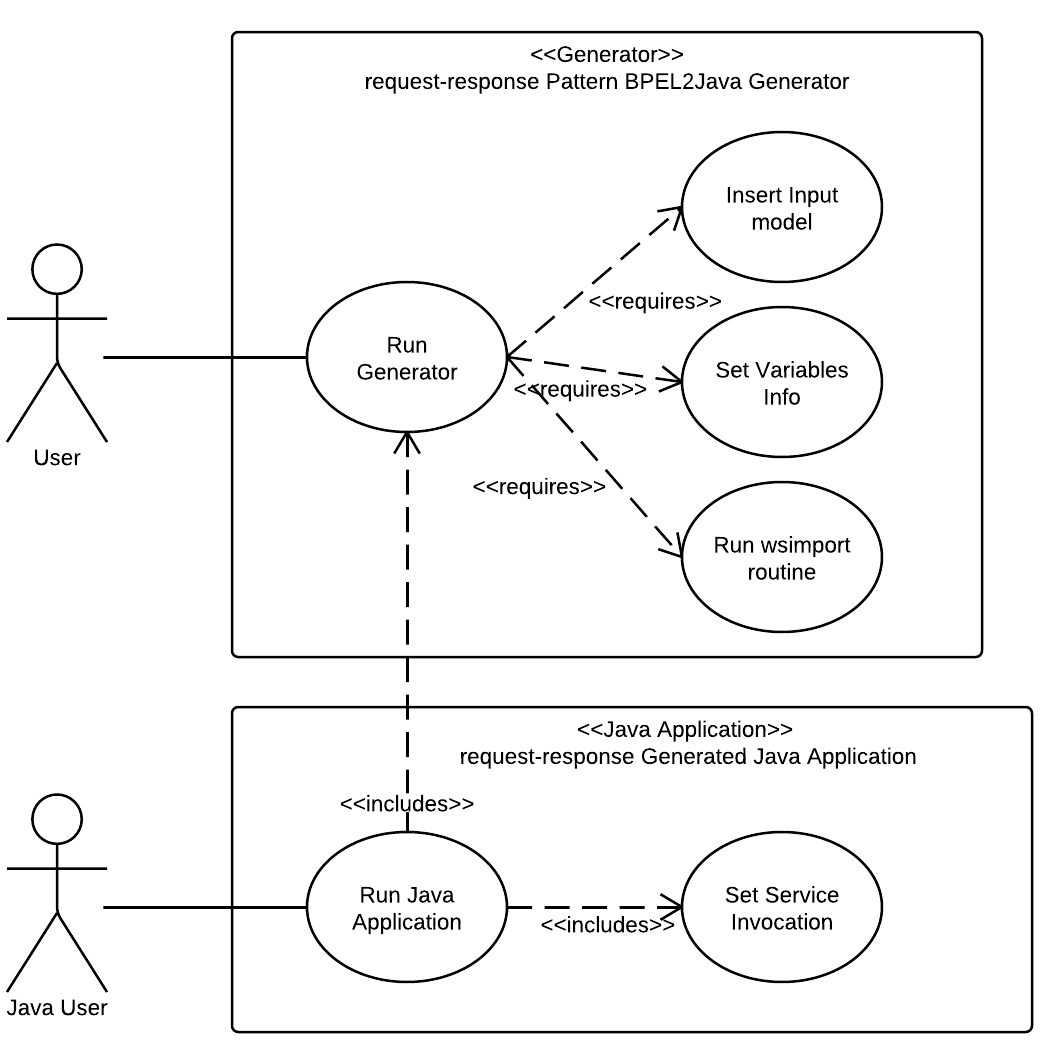
\includegraphics[scale=1.5]{pictures/GeneratorUseCase.png}
    \caption{Use Case of the BPEL to Java generator}
    \label{fig:GeneratorUseCase}
  \end{center}
\end{figure}

\subsubsection{A use case example}
As an example of how to use our transformation, we discuss in this Subsection how the behavior of a simple BPEL process is translated in Java. Figure \ref{fig:BPELOrchestr} shows the simple BPEL orchestration we provide as input to the generator. A user wants to retrieve the signature of a famous person given his surname. The BPEL process, receives the surname from the user and invokes a web server that shows an operation (\textit{getAutograph(String)}). The web server checks its database and sends the complete autograph of the person (or an error if the autograph is not present) to the BPEL process. At the end, the BPEL process replies to the client providing the autograph.
\begin{figure}
  \begin{center}
    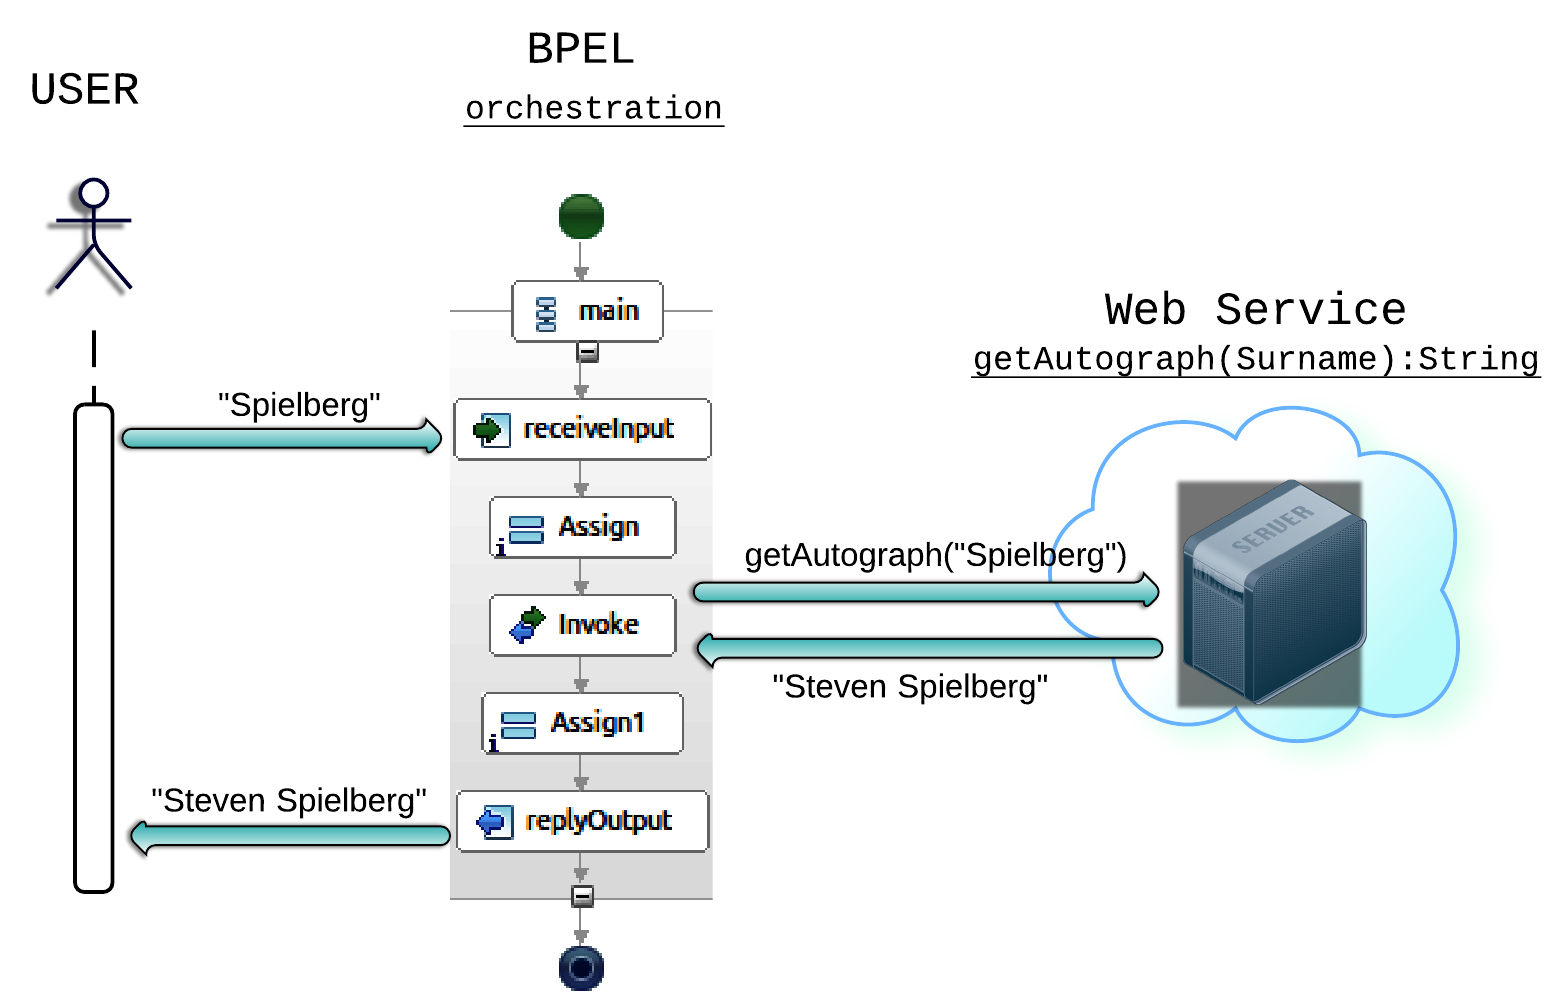
\includegraphics[scale=1.2]{pictures/UseCaseExampleBPELOrchestr.png}
    \caption{The BPEL orchestration model we input to our generator. A client uses a very simple service that, given a surname of a famous person, replies back the autograph.}
    \label{fig:BPELOrchestr}
  \end{center}
\end{figure}

Once we have the BPEL process model, its components' WSDL descriptions (one for the client and one for the web service), we can start a generation. Following Figure \ref{fig:GeneratorUseCase}, the use case shows that to run the generator we are required three things: a) provide the BPEL input model, b) manually set the variables information taken from the WSDL file, c) run the \textit{wsimport} routine on the WSDL descriptors to get the correspondent Java structure.
Once the generator has run, we obtain a Java application that mimics the given BPEL workflow. The sequence diagram depicted in Figure \ref{fig:GeneratorSequenceDiagram} shows how the behaviour of the BPEL process of Figure \ref{fig:BPELOrchestr} is emulated. This sequence diagram only shows the most important interactions among the main participants, namely, the Process class, the Client partnerLink, the Web Service partnerLink and the real Web Service running on some servers. 
We observe that the Process class (with its \textit{runWorkflow()} method, as explained in Section \ref{sec:mimicBPELLogic}) takes care of simulating the actions performed by the BPEL process. At first it creates the partnerLinks STUBS instances: PLClient and PLWebService (which inside contain the variables related their correspondent partnerLinks). Later, the Process class, with synchronous calls, starts a sequence including the following steps:
\begin{itemize}
 \item receives the input from the PLClient class (to stick to the previous example, we can imagine the user has inserted the surname "Spielberg")
 \item sets the private variables containing the input for the web service in the PLWebService class
 \item calls the \textit{getAutographBySurnameEasyStub()} method.
 \item the PLWebService class is in charge to forward the call to the real Web Service. It calls its operation to retrieve the autograph: \textit{getAutograph("Spielberg")}
 \item the Web Service response ("Steven Spielberg") is intercepted and forwarded back to the Process class
 \item the process class sets the result variable in the PLClient class
 \item the process class calls the \textit{replyOutput()} method on the PLCLient STUB class, to give back the result ("Steven Spielberg") to the user.
 \item the STUB objects are destroyed and the process has finished.
\end{itemize}

We could easily see the similarities between the BPEL process behaviour (in Figure \ref{fig:BPELOrchestr}) and the Java application logic (in Figure \ref{fig:GeneratorSequenceDiagram}). They both end up providing a response to a user willing to use the \textit{getAutograph()} web service, using though, very different approaches and frameworks to be run on.


\begin{figure}
  \begin{center}
    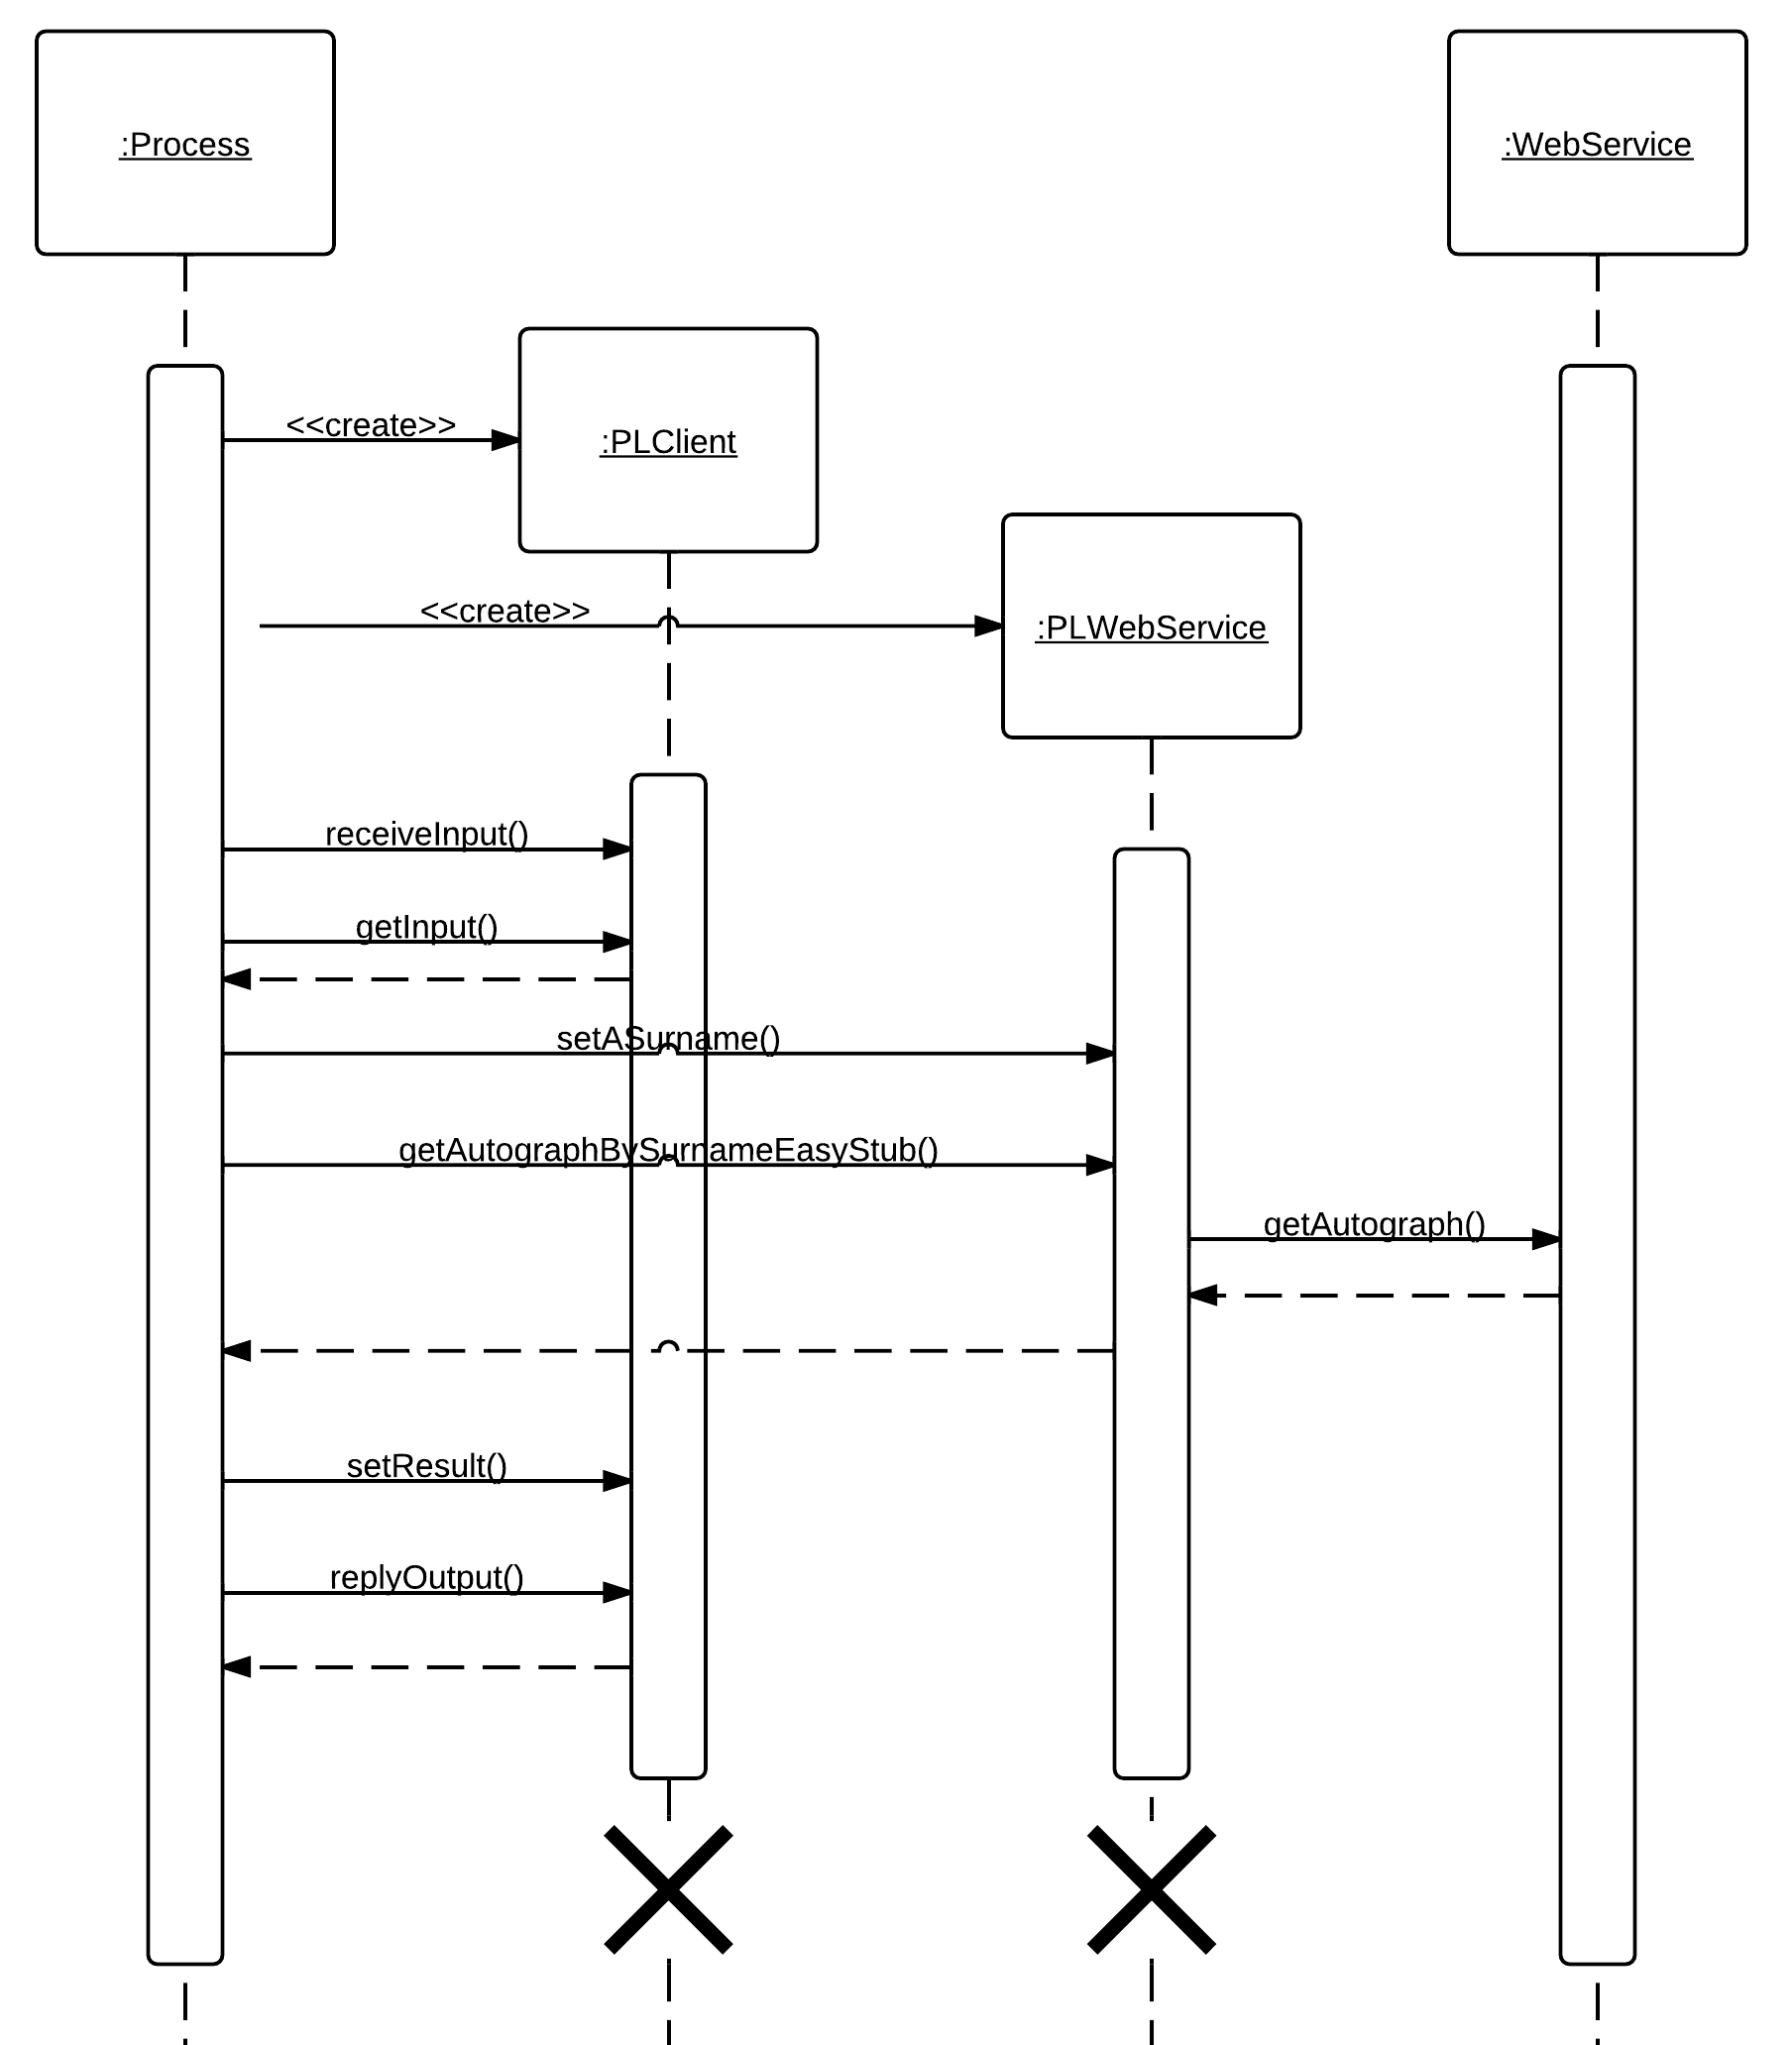
\includegraphics[scale=1]{pictures/GeneratorSequenceDiagram.png}
    \caption{Sequence diagram representing the generated Java application behaviour correspondent to the BPEL process model provided as input to the generator.}
    \label{fig:GeneratorSequenceDiagram}
  \end{center}
\end{figure}


\subsection{Future Development}
\label{sec:FutureDevelopment}
This Section briefly shows the possible improvements and future development that might be carried out on the BPEL to Java transformation.

\subsubsection{Retrieve information from WSDL files}
\label{sec:FutRetrieveWSDLInfo}
As previously described in Section \ref{sec:issues}, some technical issues mainly due to the impossibility of providing more than one input models to the Acceleo generator, made us redefine the design and contemplate a developer's intervention 
for anything that concern the WSDL files.
We think that if the information from the WSDL file would be available, the developer's intervention would be much less needed, and error-prone manual operations (like rewriting or copy-pasting the, often long, WSDL elements fields) would be avoided. 
We forecast a possible future development undertaking two ways:
\begin{enumerate}
 \item \label{itm:num1}modify the Acceleo API and implementation
 \item \label{itm:num2}recur to Java properties file 
\end{enumerate}

\paragraph{Modify the Acceleo tool}
Concerning the point number \ref{itm:num1}, modifications to the Acceleo API and its implementation could be made, though at a high cost in terms of time and knowledge to acquire concerning the Acceleo's internal mechanisms. As the Acceleo developers responded us on the official forum: the modifications would not be a trivial task.
Moreover, we don't know if the developers would take into considerations the option of rising the number of possible input files. This because the majority of Acceleo users tend to run the same transformation over several input models of the same kind (e.g. batch transformation of UML diagrams in Java) while a case like ours, where coordination among input models is required (BPEL and WSDL files), it is not common.

\paragraph{Java properties file}
A simpler idea to overcome the problem of accessing the WSDL file would be to create another Acceleo transformation (parameterized by the WSDL meta-model) taking as input a WSDL file. From here we could get the needed information and write them out in a Java Properties file. A Java properties file, as shown in the Listing \ref{lis:JavaPropertyFile}, is a very simple text file containing some variables and their values. It is usually provided to a Java application when some parameters have to be set manually, like, for example, the absolute path to some local resources.

\begin{center}
  \begin{minipage}{1\textwidth}
    \begin{java-code}{Example of a Java properties file}{lis:JavaPropertyFile}
#Mon Aug 31 12:50:43 GMT 2012
ElementType=Person
ElementName=Employee
database=localhost
user=process
    \end{java-code}
  \end{minipage}
\end{center}

Once we would have written the information from the WSDL file in the Java properties file, we could use the Acceleo facility that permits to input a Java properties file with the command:\\
\begin{verbatim}[getProperty('myProperty')/]\end{verbatim} 
The usage of properties file in Acceleo is described in the documentation \cite{acceleoDoc}. If the WSDL files are more than one (e.g. presence of more than one PartnerLink), the transformations could be run more times attaching the new information at the end of the properties file.
This improvement would basically overcome both the issues presented in Section \ref{sec:issues}.

\subsubsection{Include more BPEL patterns}
\label{sec:FutMorePatterns}
Our transformation focuses on only one kind of BPEL workflow patten, namely, a sequence of "receive - assign - invoke - assign - reply". More patterns could be added, especially working on simple variants of some basic ones. A good source of information on workflow patterns, is the Article from W.M.P. Vand Der Aalst et. al. \cite{AalstHKB03}; here the workflow patterns are abstracted from the modeling tools, so that they can be generalized, spotting commonalities and differences among them.
Eventually, transformations addressing different workflow patterns could be, either contained in their own generator, or be a specialization of another pattern. For example, a pattern where a final reply must be sent to two PartnerLinks (two BPEL \textit{reply}s), could be a special case of the one where there is only one reply to one PartnerLink.    

\subsubsection{Improve architectural design for additional Patterns}
\label{sec:FutImproveArchitectDesign}
Once the set of BPEL patterns would be enlarged, it will be necessary to improve the code reuse and add some abstraction layers to the architecture of both the Acceleo transformation and the Java application. Some of the ideas could be to use Acceleo modules hierarchies (see Table \ref{tab:terminology} on the Acceleo terminology) to specialize some of the operations. For example, one could be in need to create different PartnerLink STUBs depending on the type or role of the PartnerLink. The same happens with the Java application, where PartnerLinks STUBS could be implementing a generic PartnerLink interface class. 
